\documentclass[tikz,border=10pt]{standalone}
\usepackage{tikz}
\begin{document}
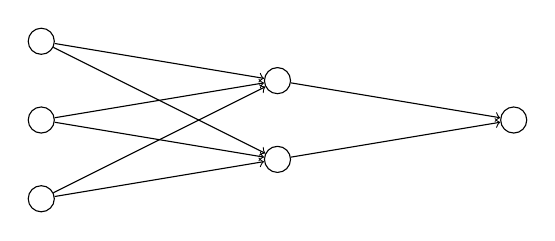
\begin{tikzpicture}[x=1.5cm, y=1cm]
  \foreach \y in {0,1,2} \node[draw, circle] (i\y) at (0,\y) {};
  % Node names must not contain dots (TikZ reads "h0.5" as anchor "5" of "h0").
  \foreach \y/\n in {0.5/1, 1.5/2} \node[draw, circle] (h\n) at (2,\y) {};
  \node[draw, circle] (o) at (4,1) {};
  \foreach \i in {0,1,2} \foreach \h in {1,2} \draw[->] (i\i) -- (h\h);
  \foreach \h in {1,2} \draw[->] (h\h) -- (o);
\end{tikzpicture}
\end{document}
